
\newpage
{\bfseries МРНТИ 20.15.13}

{\bfseries МОДЕЛИРОВАНИЕ ЦИФРОВЫХ БИЗНЕС-ПРОЦЕССОВ В ОБРАЗОВАТЕЛЬНЫХ
УЧРЕЖДЕНИЯХ}

{\bfseries А.Тельман, Д.Р.Рашидинов\textsuperscript{🖂}}

Международный университет информационных технологий, г. Алматы,
Казахстан

{\bfseries \textsuperscript{🖂}}Корреспондент-автор: damir.dmr88@gmail.com

Цифровизация затрагивает бизнес-процессы в сервисных организациях и
проявляется через внедрение цифровых технологий для повышения их
эффективности. Это ведет к изменению бизнес-процессов и, в некоторых
случаях, к полной трансформации бизнес-модели компании. Экономисты и
специалисты прогнозируют, что такие изменения будут касаться всех
компаний в будущем.

Целью данного исследования является улучшение и внедрение методов
цифровизации бизнес-процессов в образовательных центрах для оптимизации
их работы, увеличения производительности и улучшения взаимодействия с
клиентами. В статье анализируется природа цифровизации в образовании и
рассматривается применение цифровизации в бизнес-процессах
образовательных учреждений.

В ходе исследования были выделены ключевые современные инструменты для
эффективного моделирования бизнес-процессов, которые помогают повысить
эффективность и конкурентоспособность бизнес-процессов, а также общую
производительность компании на фоне цифровизации. В рамках работы также
разработана методика оценки эффективности моделирования бизнес-процессов
в условиях цифровизации.

{\bfseries Ключевые слова:} цифровизация образования, цифровизация
процессов, улучшение процессов, образование, бизнес-процессы.

{\bfseries БІЛІМ ОРЫНДАРЫНДАҒЫ ЦИФРЛЫҚ БИЗНЕС-ПРОЦЕСТЕРДІ МОДЕЛЬДЕУ}

{\bfseries А.Тельман, Д.Р. Рашидинов\textsuperscript{🖂}}

Халықаралық ақпараттық технологиялар университеті, Алматы, Қазақстан,

e-mail:damir.dmr88@gmail.com

Цифрландыру сервистік ұйымдардағы бизнес-процестерге әсер етеді және
олардың тиімділігін арттыру үшін цифрлық технологияларды енгізу арқылы
көрінеді. Бұл бизнес-процестердің өзгеруіне және кейбір жағдайларда
компанияның бизнес моделінің толық өзгеруіне әкеледі. Экономистер мен
сарапшылар мұндай өзгерістер болашақта барлық компанияларға әсер етеді
деп болжайды.

Бұл зерттеудің мақсаты -- білім беру орталықтарында олардың жұмысын
оңтайландыру, өнімділікті арттыру және клиенттермен өзара әрекеттесуді
жақсарту үшін бизнес-процестерді цифрландыру әдістерін жетілдіру және
енгізу. Мақалада білім берудегі цифрландырудың табиғаты талданып, білім
беру ұйымдарының бизнес-процестерінде цифрландыруды қолдану мәселелері
талқыланады.

Зерттеу бизнес-процестердің тиімділігі мен бәсекеге қабілеттілігін,
сондай-ақ цифрландыру аясында компанияның жалпы жұмысын жақсартуға
көмектесетін бизнес-процестерді тиімді модельдеудің негізгі заманауи
құралдарын анықтады. Жұмыс аясында цифрландыру жағдайында
бизнес-үдерістерді модельдеу тиімділігін бағалау әдістемесі де
әзірленді.

{\bfseries Түйін сөздер:} білім беруді цифрландыру, процестерді
цифрландыру, үдерістерді жетілдіру, білім беру, бизнес-процестер.

{\bfseries MODELING DIGITAL BUSINESS PROCESSES IN EDUCATIONAL INSTITUTIONS}

{\bfseries A.Telman, D.R.Rashidinov\textsuperscript{🖂}}

International University of Information Technologies, Almaty,
Kazakhstan,

e-mail:damir.dmr88@gmail.com

Digitalization affects business processes in service organizations and
manifests itself through the introduction of digital technologies to
improve their efficiency. This leads to changes in business processes
and, in some cases, to a complete transformation of the
company\textquotesingle s business model. Economists and experts predict
that such changes will affect all companies in the future.

The purpose of this study is to improve and implement methods of
digitalization of business processes in educational centers to optimize
their work, increase productivity and improve interaction with
customers. The article analyzes the nature of digitalization in
education and considers the application of digitalization in the
business processes of educational institutions.

The study identified key modern tools for effective modeling of business
processes that help improve the efficiency and competitiveness of
business processes, as well as the overall performance of the company
against the background of digitalization. As part of the work, a
methodology for assessing the effectiveness of business process modeling
in the context of digitalization was also developed.

{\bfseries Key words:} digitalization of education, digitalization of
processes, process improvement, education, business processes.

{\bfseries Введение.} Современная цифровая революция разворачивается с
поразительной скоростью. Если переход от громоздких компьютеров к
персональным устройствам занял десятилетия, то новые технологические
модели могут меняться всего за несколько месяцев. Изначально
цифровизация охватывала автоматизацию бизнес-процессов, улучшение
доступа в Интернет, развитие социальных сетей и внедрение новых
устройств, таких как планшеты и смартфоны. Сейчас, с ускорением
цифровизации, технологии становятся неотъемлемой частью повседневной
жизни, включая сферу образования.

Цифровизация в образовании требует кардинальных изменений, так как
преподаватели должны адаптироваться к новым технологиям и эффективно их
использовать. Например, виртуальная реальность (VR) позволяет создавать
цифровые миры и симуляции, которые не подчиняются физическим
ограничениям. Это расширяет возможности обучения, а дистанционное
образование предоставляет доступ к образовательным ресурсам в любое
время и из любой точки мира.

Сегодня информация является краеугольным камнем глобального прогресса,
что делает традиционные подходы неадекватными. Как подчеркивает Л.В.
Шмелькова, важнейшей характеристикой людей, подходящих для цифровой
экономики, является их владение цифровыми технологиями и их применение в
профессиональной деятельности {[}1{]}.

Дети, которые приобрели навыки общения в цифровой среде за пределами
формального образования, особенно уязвимы перед последствиями оцифровки.

В то время как конкретным навыкам обучают на разных уровнях образования,
цифровые компетенции постоянно приобретаются и обновляются на протяжении
всей жизни. Таким образом, цифровизация образования тесно связана с
владением наставниками современными технологиями, поскольку им
необходимо эффективно внедрять их в образовательный процесс. Н.Н.
Битюцкая подчеркивает важность того, чтобы учителя приобрели навыки
ориентировки в потоке цифровой информации, умели работать с ней,
обрабатывать и интегрировать в новые технологии {[}2{]}. Система
цифрового образования состоит из таких элементов, как: информационные
ресурсы, телекоммуникации и управляющая система (рис. 1).

\begin{figure}[H]
	\centering
	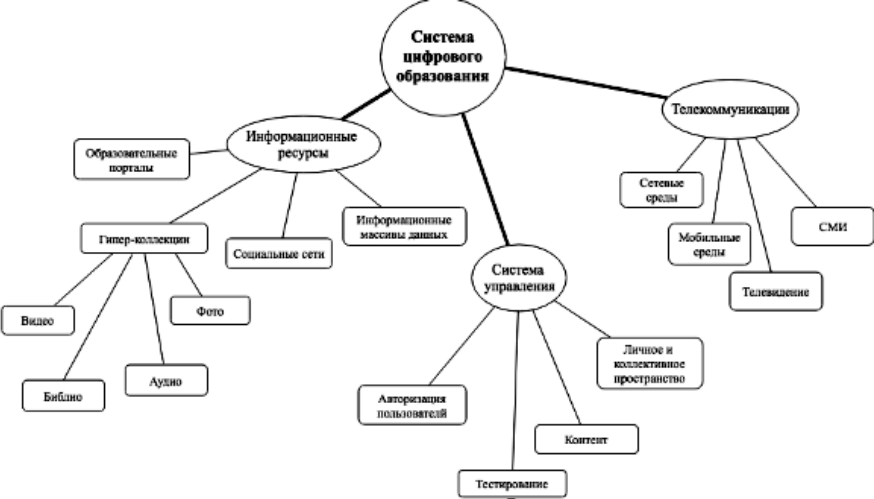
\includegraphics[width=0.8\textwidth]{assets/205}
	\caption*{}
\end{figure}

{\bfseries Рис. 1 -- Составляющие системы цифрового образования}

{\bfseries Материалы и методы.} Использование новых технологий, механизмов
и алгоритмов в образовательном процессе требует их эффективного
использования. Дистанционное и смешанное обучение предоставляют людям
огромные возможности для доступа к качественному образованию, независимо
от их географического положения и имеющихся навыков, а также с учетом их
конкретных требований и возможностей.

Эти изменения требуют, чтобы учителя обладали всесторонним пониманием
цифровой сферы. Поэтому крайне важно установить "единые стандарты для
уже существующих и разрабатываемых онлайн-курсовых платформ, чтобы они
могли быть интегрированы в единую систему, аналогичную "единому окну".

Условия для оцифровки можно сформулировать следующим образом:

1. всеобщий доступ: физические лица и организации на всей территории
Казахстана, независимо от их местонахождения, должны иметь доступ к
информационным ресурсам и возможностям, необходимым для их личной и
деловой деятельности, бесплатно или за плату

2. доступность технологий: общество должно обеспечить свободный доступ к
соответствующим цифровым технологиям и обеспечить практическую
реализацию вышеуказанных условий

3. развитие инфраструктуры: должна быть создана достаточная
инфраструктура для поддержки национальных информационных ресурсов,
необходимых для развития быстро эволюционирующего общества. Общество
должно генерировать и хранить всю информацию, необходимую для его
функционирования, в частности научные знания.

4. автоматизация: должна происходить непрерывная автоматизация всех сфер
экономической и социальной жизни общества.

5. глобальное влияние: расширение цифровой деятельности и
информационно-коммуникационных услуг происходит под влиянием глобальной
трансформации социальных структур.

В последнее время разработка и использование открытых онлайн-ресурсов
набрали значительный импульс. Это включает в себя целый ряд ресурсов, от
индивидуальных заданий и тестов до комплексных курсов и модулей,
направленных на формирование необходимых компетенций. Растущая
доступность онлайн-курсов свидетельствует о динамичном развитии
онлайн-обучения.

Цифровизация образования выходит за рамки онлайн-курсов и включает в
себя развитие цифровых библиотек и виртуальных университетских городков.
Создание и внедрение онлайн-курсов предполагает использование
программных решений, которые позволяют собирать курсы из существующих
информационных ресурсов и специализированных программных сред.

Образование играет решающую роль в развитии интеллекта людей и
обеспечении их возможности трудоустройства в эпоху цифровых
преобразований. Это считается одним из основных принципов, с помощью
которых развиваются и совершенствуются навыки сотрудников. Осваивая
цифровизацию, школьники и студенты могут получить более глубокое
представление о реальном мире, особенно о современных технологиях
{[}3{]}.

Исследования показывают, что уже 37 процентов образовательных
организаций по всему миру применяют искусственный интеллект, включая
чат-ботов, для учебного процесса {[}4{]}. Студенты и ученики высоко
оценивают взаимодействие с программой и считают, что она способствует
лучшему обучению, по сравнению с человеком. Теперь давайте разберемся,
что представляют собой чат-боты и почему они востребованы в образовании.

На основании исследования использования чат-ботов в образовательном
процессе, можно выделить следующие рекомендации для повышения их
эффективности:

\begin{enumerate}
\def\labelenumi{\arabic{enumi}.}
\item
  Преимущества использования Telegram-ботов в образовании:

  \begin{itemize}
  \item
    Быстрая коммуникация между студентами и преподавателями.
  \item
    Участие и вовлеченность в образовательный процесс.
  \item
    Удобное хранение материалов курса и работ студентов.
  \item
    Отсутствие необходимости загружать дополнительные приложения.
  \item
    Бесплатное использование.
  \end{itemize}
\item
  Недостатки использования Telegram-ботов в образовании:

  \begin{itemize}
  \item
    Возможное увеличение нагрузки на преподавателя.
  \item
    Отвлечение студентов от основных тем обсуждения или взаимодействие с
    другими участниками чата.
  \item
    Необходимость наличия смартфона с доступом в интернет.
  \item
    Возможная потеря информации, хранящейся на мобильных устройствах.
  \end{itemize}
\item
  Чат-боты в образовании должны быть простыми, быстрыми в поиске
  информации и обеспечивать безопасный доступ к ней. Их интерфейс должен
  быть понятным и удобным для пользователей. Такие инструменты
  коммуникации помогут ускорить и упростить взаимодействие между
  студентами и преподавателями, экономя время.
\item
  Чат-боты могут использоваться для проведения тематических
  онлайн-квестов, предоставления нового материала и развития
  коммуникации между преподавателями и студентами. Они также могут
  способствовать вовлечению студентов в новые формы обучения и
  познавательной деятельности.
\end{enumerate}

Одним из основных преимуществ чат-ботов является их широкая
популярность. Отправка сообщений через мессенджеры удобна и не создает
дополнительной нагрузки на приложение. Коммуникация в чат-ботах краткая,
информативная и быстрая. Благодаря этому педагоги могут быстро и легко
устанавливать контакт с учениками и своевременно передавать им всю
важную информацию {[}5{]}.

Эффективность взаимодействия и коммуникации между преподавателями и
учениками, адаптация к изменяющимся условиям и успешное внедрение новых
технологий в образовательный процесс влияют на развитие системы
образования и государства в целом {[}6{]}.

{\bfseries Обсуждение и результаты.} При цифровизации бизнес-процессов и
внедрении чат-бота в организацию необходимо оценить их эффективность и
целесообразность. Для этого можно использовать язык моделирования
бизнес-процессов BPMN (Business Process Model and Notation), который
поможет описать и визуализировать процессы и их реализацию в различных
системах управления.

BPMN является составной частью двух основных компонентов:

- BPM (бизнес-процессное моделирование) - это среда, в которой вы
активно участвуете в создании моделей, как в одиночку, так и в команде.

- BPMS (система моделирования бизнес-процессов) - это инструменты,
которые позволяют выполнить созданные вами модели. Примерами таких
инструментов являются Bizagi, Comundo, ELMA и другие.

Создание BPMN-диаграммы для образовательного центра требует знаний в
области бизнес-анализа; BPMN-модель не ограничивается простыми
картинками и диаграммами, которые можно нарисовать в графическом
редакторе. Важным аспектом является правильная структура и
последовательность процессов.

Чтобы показать, как принципы бизнес-моделирования реализуются в
событийно-процессной нотации, рассмотрим пример процесса, который входит
в контракт курса бизнес-анализа в современной образовательной школе.

\begin{enumerate}
\def\labelenumi{\arabic{enumi}.}
\item
  Процесс начинается с того, что заказчик оставляет заявку на сайте.
\item
  На основании заявки менеджер формирует коммерческое предложение,
  которое, в зависимости от предоставленных контактных данных,
  озвучивается по телефону или отправляется на электронную почту
  клиента.
\item
  Клиент принимает решение на основании предложения. Если клиент не
  желает проходить обучение, процесс работы с ним завершается.
\item
  Если клиент согласен с условиями, он сообщает менеджеру о своем
  намерении заключить договор и предоставляет необходимые данные.
\item
  Менеджер готовит проект договора и отправляет его клиенту на
  согласование.
\item
  Если у клиента нет возражений, договор подписывается, и процесс
  заключения договора завершается. Начинается процесс оплаты, который
  описан на другой схеме.
\item
  Если по проекту договора есть возражения, клиент вносит изменения и
  отправляет его менеджеру.
\end{enumerate}

Менеджер готовит новый проект договора и отправляет его обратно клиенту
на утверждение, повторяя шаги 5-7.

Чтобы улучшить понимание диаграммы, мы разделили процесс на две части:
обработку заявки и заключение договора. Клиента представляем внешним
закрытым пулом, с которым взаимодействуем через потоки сообщений. Для
компактного размещения элементов диаграммы мы предусмотрели обход потока
сообщений между пулами, чтобы избежать пересечений линий и упростить
диаграмму (рис. 2).

\begin{figure}[H]
	\centering
	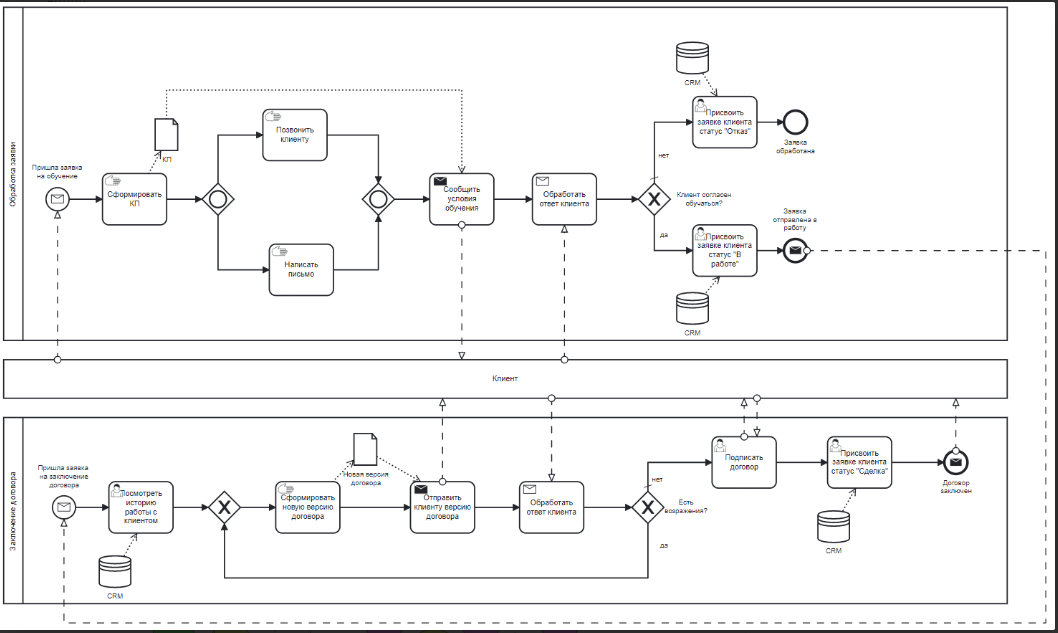
\includegraphics[width=0.8\textwidth]{assets/206}
	\caption*{}
\end{figure}

{\bfseries Рис. 2 -- BPMN-диаграмма для образовательного центра}

В ходе работы был разработан соответствующий алгоритм (рис.3) для оценки
эффективности моделирования бизнес-процессов компании в условиях
цифровизации. Этот алгоритм представляет собой подробную схему с
определенными вариантами исполнения этапов и принимаемых решений,
включая как положительные, так и отрицательные их развития. Все это
отображено в графическом виде.

\begin{figure}[H]
	\centering
	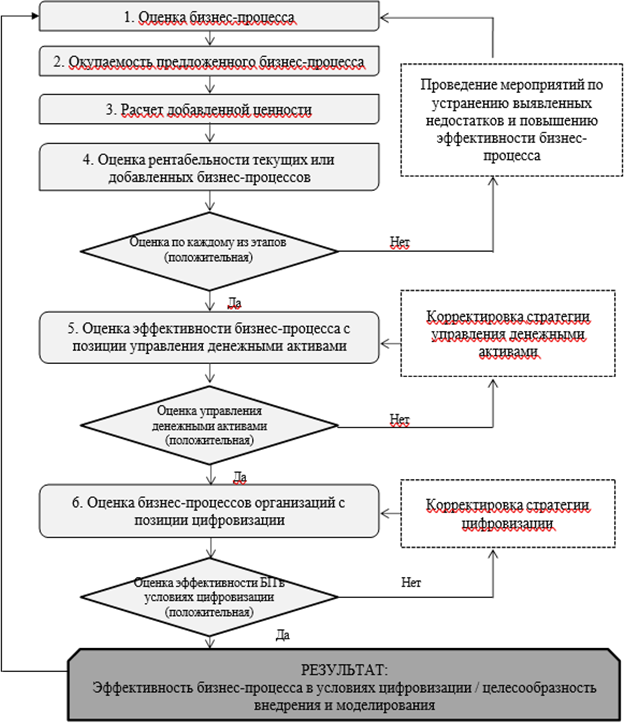
\includegraphics[width=0.8\textwidth]{assets/207}
	\caption*{}
\end{figure}

{\bfseries Рис. 3 -- Алгоритм оценки эффективности моделирования бизнес-
процессов компании в условиях цифровизации}

Алгоритм оценки эффективности моделирования бизнес-процессов компании в
условиях цифровизации, начинается с исследования бизнес-процесса, его
организации, степени выполнения, в том числе общей оценки. Следующим
этапом в предложенной методике является оценка окупаемости предложенного
бизнес-процесса. Данный этап является расчетным, расчет окупаемости
предложенного бизнес-процесса осуществляется по формуле (1):

ПО = ИС / ДПn (1)

где ПО -- период окупаемости предложенного бизнес-процесса;

ИС -- сумма инвестиционных средств, которые направлены на реализацию
предлагаемого бизнес-процесса, тыс.тг.;

ДПn -- средняя сумма денежного потока от реализации предлагаемого
бизнес-процесса, (заработная плата одного оператора) тыс.тг.;

n -- количество периодов, в данном случае 1.

ПО = 1600 / 170 *12 = 0,76 года = 8 мес.

Характеризуя вышеуказанный показатель, следует обратить внимание на то,
что он может быть использован для оценки не только эффективности
предлагаемого бизнес-процесса, но и уровня рисков.

Последующим этапом в алгоритме оценки эффективности моделирования
бизнес-процессов компании в условиях цифровизации является расчет
добавленной стоимости.

Добавленная ценность служит теоретической концепцией, которая выражает
соотношение рыночной стоимости и фактически понесенных затрат от
предлагаемого бизнес-процесса. Величину добавленной ценности (AV) можно
рассчитать по формуле (2):

AV = Va -- Vb (2)

Va -- ценность бизнес-процесса после обработки;

Vb -- ценность бизнес-процесса перед обработкой.

AV = 3~656~000 -- 3~000~000 = 656 тыс. тг

С целью оценки эффективности моделирования бизнес-процессов, которые
добавляют экономическую ценность (затраты), на отдельном бизнес-
процессе данную ценность можно выразить в виде определенного удельного
показателя.

Оценка рентабельности текущих или добавленных бизнес-процессов --
следующий этап в разработанном алгоритме оценки эффективности
моделирования бизнес-процессов компании в условиях цифровизации. Данный
показатель является относительным уровнем прибыльности от предлагаемого
бизнес-процесса в компании.

Рентабельность текущих или добавленных бизнес-процессов (Р)
рассчитывается по формуле (3):

P = П / В (3)

П -- прибыль от текущих или добавленных бизнес-процессов в организации,
тыс.тг.;

В -- выручка от текущих или добавленных бизнес-процессов в организации,
тыс.тг..

P = 1200 / 2450 =0,49 = 49\%

В условиях получения оптимального значения (более 4\%), повышения его в
динамике (в сравнении с текущим показателем, то есть показателем
отчетного периода), необходимо перейти к следующему этапу в
разработанной методике. В условиях значения до 4\%, сокращения его в
динамике, следует проводить мероприятия по устранению выявленных
недостатков и повышению эффективности моделирования бизнес-процесса в
компании, чтобы впоследствии вернуться к этапу и перейти к последующему
по разработанной методике {[}7{]}.

Оценка эффективности бизнес-процесса с позиции управления денежными
активами -- пятый этап в алгоритме оценки эффективности моделирования
бизнес-процессов компании в условиях цифровизации. На данном этапе
проводится расчет по основным показателям эффективности: степени участия
денежных активов бизнес-процессов в совокупных оборотных активах
организации, среднему периоду оборота и количества оборотов денежных
активов бизнес-процессов в рассматриваемом периоде, количеству оборотов
среднего остатка денежных активов в рассматриваемом периоде для бизнес-
процессов, коэффициенту рентабельности краткосрочных финансовых
инвестиций для бизнес-процессов, а также планируемой суммы операционного
остатка денежных активов бизнес-процессов (табл. 1).

{\bfseries Таблица 1 -- Показатели эффективности моделирования
бизнес-процесса с позиции управления денежными активами}

\begin{longtable}[]{@{}
  >{\raggedright\arraybackslash}p{(\columnwidth - 4\tabcolsep) * \real{0.2722}}
  >{\raggedright\arraybackslash}p{(\columnwidth - 4\tabcolsep) * \real{0.3070}}
  >{\raggedright\arraybackslash}p{(\columnwidth - 4\tabcolsep) * \real{0.4207}}@{}}
\toprule\noalign{}
\begin{minipage}[b]{\linewidth}\raggedright
Наименование показателя
\end{minipage} & \begin{minipage}[b]{\linewidth}\raggedright
Сущность показателя
\end{minipage} & \begin{minipage}[b]{\linewidth}\raggedright
Расчет (формула с пояснениями)
\end{minipage} \\
\midrule\noalign{}
\endhead
\bottomrule\noalign{}
\endlastfoot
Степень участия денежных активов бизнес-процессов в совокупных оборотных
активах организации (КУ) & Показывает степень участия денежных активов
предприятия в оборотном капитале в условиях реализации бизнес-процессов
& {\bfseries КУ = ДА / ОА}

ДА -- средний остаток совокупных денежных активов, тыс.тг.;

ОА -- средняя сумма оборотных активов организации, тыс.тг. \\
Средний период оборота и количество оборотов денежных активов бизнес-
процессов в рассматриваемом периоде (ПО) & Показывает степень
оборачиваемости активов в условиях реализации бизнес- процессов &
{\bfseries пО = ДА / РДА}

РДА -- однодневный объем расходования денежных средств, тыс.тг. \\
Количество оборотов среднего остатка денежных активов в рассматриваемом
периоде для бизнес- процессов (КО) & Показывает степень оборачиваемости
среднего остатка денежных активов & {\bfseries КО = РДАо / ДА}

РДАо -- общий объем расходования денежных средств, тыс.тг. \\
Коэффициент рентабельности краткосрочных финансовых инвестиций для
бизнес-процессов (КРкфи) & Показывает степень прибыльности краткосрочных
финансовых инвестиций для бизнес-процессов, то есть экономическую
целесообразность их ввода & {\bfseries КРкфи = П / КФИ}

П -- сумма прибыли, которая получена организацией от инвестирования,
тыс.тг. \\
Планируемая сумма операционного остатка денежных активов
бизнес-процессов (Дао) & Показывает потребность в остатках денежных
активов бизнес-процессов в условиях реализации бизнес-процессов &
{\bfseries ДАо = пО / КО}

пО -- планируемый объем отрицательного денежного потока, тыс.тг.;

КО -- количество оборотов среднего остатка денежных активов по плану. \\
\end{longtable}

Также как и было указано ранее, при положительной оценке бизнес-
процесса с позиции управления денежными активами (приросте в динамике,
например в сравнении с отчетными показателями), выполняется следующий
этап, а при сокращении, небольших значениях -- происходит корректировка
существующей или выбранной стратегии управления денежными активами в
компании, чтобы также вернуться к данному этапу, достичь запланированных
целей и задач.

{\bfseries Выводы.} Существует множество подходов и принципов для
модернизации образовательного процесса. Одним из ключевых аспектов
является мотивация и заинтересованность учеников. Быстрые
технологические изменения существенно изменили ожидания детей от
учебного процесса. Традиционные методы уже не вызывают у них интерес,
поэтому педагогам необходимо адаптироваться к современным требованиям и
искать новые подходы в обучении.

Эта тенденция вынуждает учителей искать инновационные методы работы,
что, в свою очередь, предоставляет им возможность развиваться, улучшать
свои педагогические навыки и открывает новые горизонты для преподавания.
Правильно подобранные методы обучения помогают учителям завоевать
уважение учеников и поддерживать их интерес к учебе.

Быстрые изменения в обществе требуют оперативной адаптации методов
преподавания. Чем быстрее учителя осваивают новые возможности и
учитывают потребности учеников, тем более эффективным становится
образовательный процесс. Качество знаний, полученных в школе, напрямую
влияет на уровень квалификации будущих специалистов в различных
областях.

Цель данной работы заключалась в разработке и внедрении методов
цифровизации для бизнес-процессов в образовательных центрах. Это
позволит оптимизировать множество бизнес-процессов, повысить
производительность и улучшить взаимодействие с клиентами.

Анализ показал особенности моделирования бизнес-процессов в условиях
цифровизации, такие как расширение функций специалистов, использование
различных цифровых инструментов и технологий, а также автоматизация
процессов.

На основе исследования была разработана методика моделирования
бизнес-процессов с учетом цифровизации. Эта методика представляет собой
универсальный подход к изучению и оценке процессов, включающий
соответствующие факторы и инструменты для достижения целей, создания
конкурентной среды на рынке, соответствия мировым стандартам и улучшения
качества в условиях современных потребительских тенденций.

{\bfseries Литература}

1.Козлов С.В., Резванцева А.А. Чат-боты как одна из тенденций развития
современного образования // Международный журнал экспериментального
образования.-2022.-№ 5. - С. 44-49.
https://expeducation.ru/ru/article/view?id=12095~

2.Грекул В.И., Денищенко Г.Н., Коровкина Н.Л. Управление внедрением
информационных систем. Методология внедрения OneMethodology. -512 с.
2021 г., издание, ISBN 978-5-4497-0910-3

3.Антонов, Г.Д. Управление проектами организации: учебник / Г.Д.
Антонов, О.П. Иванова, В.М. Тумин. -- Москва: Инфра-М, 2018.- 244 c.
ISBN 978-5-16-01332-0

4.Гузь, Д.А. Улучшение конкурентоспособности предприятия с помощью
моделирования бизнес-процессов / Д.А. Гузь, Ю.С. Бровкова // Концепции и
модели устойчивого инновационного развития общества: сборник статей
международной научно-практической конференции. -- Омега Сайнс, 2020. -
С. 52-56.

5.Буленко, Ю.А. Структурная модель развития бизнес-процессов компании /
Ю.А. Буленко // Материалы и методы инновационных исследований и
разработок: сборник статей международной научно-практической
конференции. -- Омега Сайнс, 2019. -- С. 96-97.

6.Ктет М.А. Оценка факторов, влияющих на поведение потребителей
гостиничных услуг //диссертация кандидата экономических наук.-
Владивосток, 2020. -- 230 с.

7.Смыслова Л.В. Чат-бот как современное средство интернет- коммуникаций
// Молодой ученый. - 2018. - № 9. - С. 36-39

{\bfseries References}

1.Kozlov S.V., Rezvanceva A.A. Chat-boty kak odna iz tendencij razvitija
sovremennogo obrazovanija // Mezhdunarodnyj zhurnal
jeksperimental\textquotesingle nogo obrazovanija.-2022.-№ 5. - S. 44-49.
https://expeducation.ru/ru/article/view?id=12095

2.Grekul V.I., Denishhenko G.N., Korovkina N.L. Upravlenie vnedreniem
informacionnyh sistem. Metodologija vnedrenija OneMethodology. -512 s.
2021. ISBN 978-5-4497-0910-3

3.Antonov, G.D. Upravlenie proektami organizacii: uchebnik / G.D.
Antonov, O.P. Ivanova, V.M. Tumin. -- Moskva: Infra-M, 2018.- 244 c.
ISBN 978-5-16-01332-0

4.Guz\textquotesingle, D.A. Uluchshenie konkurentosposobnosti
predprijatija s pomoshh\textquotesingle ju modelirovanija
biznes-processov / D.A. Guz\textquotesingle, Ju.S. Brovkova // Koncepcii
i modeli ustojchivogo innovacionnogo razvitija obshhestva: sbornik
statej mezhdunarodnoj nauchno-prakticheskoj konferencii. -- Omega Sajns,
2020. - S. 52-56.

5.Bulenko, Ju.A. Strukturnaja model\textquotesingle{} razvitija
biznes-processov kompanii / Ju.A. Bulenko // Materialy i metody
innovacionnyh issledovanij i razrabotok: sbornik statej mezhdunarodnoj
nauchno-prakticheskoj konferencii. -- Omega Sajns, 2019. -- S. 96-97.

6.Ktet M.A. Assessment of factors influencing the behavior of consumers
of hotel services // dissertation of candidate of economic sciences. -
Vladivostok, 2020. - 230 p.

7.Smyslova L.V. Chat-bot kak sovremennoe sredstvo internet- kommunikacij
// Molodoj uchenyj. - 2018. - № 9. - S. 36-39

\emph{{\bfseries Сведения об авторах}}

Тельман А. Б. - магистр, Международный университет информационных
технологий, г. Алматы, Казахстан, e-mail: telmanalisher@gmail.com

Рашидинов Д.Р. -докторант, Международный университет информационных
технологий, г. Алматы, Казахстан, e-mail: damir.dmr88@gmail.com

\emph{{\bfseries Information about the authors}}

Telman A.B.- Master, International University of Information
Technologies, Almaty, Kazakhstan, e-mail: telmanalisher@gmail.com

Rashidinov D. R. - Doctoral student, International University of
Information Technologies, Almaty, Kazakhstan, e-mail:
damir.dmr88@gmail.com











\newpage
{\bfseries МРНТИ 50.43.15}

{\bfseries ПОСТРОЕНИЕ ТРАЕКТОРИЙ ДЛЯ БЕСПИЛОТНЫХ АППАРАТОВ С ИСПОЛЬЗОВАНИЕМ
ПРОГРАММНОГО ПАКЕТА MISSION PLANNER ДЛЯ ИССЛЕДОВАНИЯ ВОДНЫХ ОБЪЕКТОВ}

{\bfseries \textsuperscript{1,2}М.Г. Жартыбаева\textsuperscript{🖂},
\textsuperscript{1}А.Д. Алинова, \textsuperscript{1,2}Ж.О. Оралбекова,
\textsuperscript{1}Г.А. Тюлепбердинова,\\
\textsuperscript{3}Н.М. Жамишева}

\textsuperscript{1}Евразийский национальный университет им. Л. Н.
Гумилева, Астана, Казахстан,

\textsuperscript{2} Astana IT University, Астана, Казахстан,

\textsuperscript{3} «Институт законодательства и правовой информации
Республики Казахстан»

Министерства юстиции Республики Казахстан, Астана, Казахстан

{\bfseries \textsuperscript{🖂}}Корреспондент-автор: makkenskii@mail.ru

Для эффективного управления движением беспилотных летательных и
плавательных аппаратов применяется HEX Pixhawk 2.1 CUBE ORANGE+ в
комплексе с программным пакетом Mission Planner. Цель статьи заключается
в разработке эффективных методов построения траектории для БПА с целью
повышения точности и безопасности автономных миссий. Цель данного
исследования разработка и апробация методов построения траекторий для
беспилотных аппаратов, анализ движения мобильных роботов с учетом
воздействия течения. Рассматриваются различные параметры полета, такие
как высота, скорость и курс, а также методы управления БПА в
соответствии с заданными целями. Особое внимание уделяется безопасности
и настройке датчиков и устройств, необходимых для автономного полета.
Авторские результаты включают в себя разработку алгоритмов планирования
траектории, оценку влияния течения на движение робота, а также
разработку программного обеспечения для получения и обработки данных о
морском дне. Для наглядности и анализа представлены графики и
вычислительные результаты, демонстрирующие влияние скорости течения на
траекторию движения робота. Также описаны методы разработки программного
обеспечения для получения и обработки данных о глубине дна с
использованием оборудования HEX Pixhawk 2.1 CUBE ORANGE+ и
эхолокационного устройства. Полученные результаты имеют как
теоретическую, так и практическую значимость. В теоретическом аспекте
предложенные методы позволяют более эффективно управлять БППА и
анализировать их поведение в различных условиях. В практическом плане
это открывает новые перспективы для исследования морского дна и
проведения автономных миссий с высокой точностью и безопасностью.

{\bfseries Ключевые слова:} планирование траектории, навигация, управление,
беспилотный аппарат, исследование рельефа дна.

{\bfseries СУ ОБЪЕКТІЛЕРІН ЗЕРТТЕУГЕ АРНАЛҒАН MISSION PLANNER}

{\bfseries БАҒДАРЛАМАЛЫҚ ПАКЕТІН ПАЙДАЛАНА ОТЫРЫП, ДРОНДАРҒА}

{\bfseries АРНАЛҒАН ТРАЕКТОРИЯНЫ ҚҰРУ}

{\bfseries \textsuperscript{1,2}М.Г. Жартыбаева\textsuperscript{🖂},
\textsuperscript{1}А.Д. Алинова, \textsuperscript{1,2}Ж.О. Оралбекова,
\textsuperscript{1}Г.А. Тюлепбердинова,\\
\textsuperscript{3}Н.М. Жамишева}

\textsuperscript{1}Л.Н. Гумилев атындағы Еуразия ұлттық университеті,
Астана, Қазақстан,

\textsuperscript{2}Astana IT University, Астана, Қазақстан,

\textsuperscript{3}Қазақстан Республикасы Әділет министрлігінің
«Қазақстан Республикасының Заңнама

және құқықтық ақпарат институты», Астана, Қазақстан

e-mail: makkenskii@mail.ru

Ұшқышсыз ұшу және жүзетін аппараттардың қозғалысын тиімді басқару үшін
HEX Pixhawk 2.1 CUBE ORANGE+ Mission Planner бағдарламалық пакетімен
бірге қолданылады. Бұл жұмыстың мақсаты автономды миссиялардың дәлдігі
мен қауіпсіздігін арттыру үшін Ұшқышсыз жүзетін аппараттар үшін жүзу
жолдарын салудың тиімді әдістерін әзірлеу болып табылады. Бұл зерттеудің
мақсаты токтардың әсерін ескере отырып, мобильді роботтардың қозғалысын
талдай отырып, ұшқышсыз көліктердің траекторияларын құру әдістерін
әзірлеу және сынау болып табылады. Жылдамдық және бағыт сияқты жүзудің
әртүрлі параметрлері, сондай-ақ белгіленген мақсаттарға сәйкес Ұшқышсыз
жүзетін аппараттар басқару әдістері қарастырылады. Автономды жүзуге
қажетті сенсорлар мен құрылғылардың қауіпсіздігі мен конфигурациясына
ерекше назар аударылады. Автордың нәтижелеріне траекторияны жоспарлау
алгоритмдерін жасау, токтардың робот қозғалысына әсерін бағалау,
сондай-ақ теңіз түбіндегі деректерді алу және өңдеу үшін бағдарламалық
қамтамасыз етуді әзірлеу кіреді. Түсінікті және талдау үшін ағын
жылдамдығының робот траекториясына әсерін көрсететін графиктер мен
есептеу нәтижелері ұсынылған. Сондай-ақ, HEX Pixhawk 2.1 CUBE ORANGE+
жабдығы мен эхолокация құрылғысы арқылы тереңдіктің тереңдігі туралы
деректерді алуға және өңдеуге арналған бағдарламалық құралды әзірлеу
әдістері сипатталған. Алынған нәтижелердің теориялық және практикалық
маңызы бар. Теориялық аспектіде ұсынылған әдістер ұшқышсыз жүзу
аппараттарын тиімдірек басқаруға және олардың әртүрлі жағдайларда
мінез-құлқын талдауға мүмкіндік береді. Практикалық тұрғыдан алғанда,
бұл теңіз түбін зерттеудің және жоғары дәлдікпен және қауіпсіздікпен
автономды миссияларды жүргізудің жаңа перспективаларын ашады.

{\bfseries Түйін сөздер:} траекторияны жоспарлау, навигация, басқару,
пилотсыз аппарат, төменгі рельефті зерттеу

{\bfseries CONSTRUCTING TRAJECTORIES FOR UNMANNED VEHICLES USING}

{\bfseries THE MISSION PLANNER SOFTWARE PACKAGE FOR RESEARCHING}

{\bfseries WATER BODIES}

{\bfseries \textsuperscript{1,2}M.G.}
{\bfseries Zhartybayeva\textsuperscript{🖂}, \textsuperscript{1}A.D.
Alinova, \textsuperscript{1,2}Zh.O.} {\bfseries Oralbekova,
\textsuperscript{1}G.A.} {\bfseries Tyulepberdinova,\\
\textsuperscript{3}N.M. Zhamisheva}

\textsuperscript{1}L.N. Gumilyov Eurasian National University, Astana,
Kazakhstan,

\textsuperscript{2} Astana IT University, Astana, Kazakhstan,

\textsuperscript{3}Institute of Legislation and Legal information of the
Republic of Kazakhstan" Ministry of Justice

of the Republic of Kazakhstan, Astana, Kazakhstan

e-mail: makkenskii@mail.ru

HEX Pixhawk 2.1 CUBE ORANGE+ in combination with Mission Planner
software package is used for effective motion control of unmanned aerial
and swimming vehicles. The article aims to develop efficient methods of
flight trajectory generation for USVs to improve the accuracy and safety
of autonomous missions. This research aims to develop and validate
methods of trajectory construction for unmanned vehicles and analyze the
motion of mobile robots taking into account the impact of currents.
Different flight parameters such as altitude, velocity, and heading are
considered, as well as methods for controlling the USVs according to the
given targets. Special attention is given to safety and the
configuration of sensors and devices required for autonomous flight. The
author\textquotesingle s results include the development of trajectory
planning algorithms, evaluation of the effect of currents on the
robot\textquotesingle s motion, and development of software to acquire
and process seafloor data. Graphs and computational results
demonstrating the effect of current velocity on robot trajectory are
presented for visualization and analysis. Software development methods
for acquiring and processing seabed depth data using HEX Pixhawk 2.1
CUBE ORANGE+ hardware and an echolocation device are also described. The
obtained results have both theoretical and practical significance. In
the theoretical aspect, the proposed methods allow us to control USVs
more efficiently and analyze their behavior in different conditions. In
practical terms, it opens new perspectives for seabed exploration and
autonomous missions with high accuracy and safety.

{\bfseries Key words:} trajectory planning, navigation, control, unmanned
aerial vehicle, bottom relief research.

{\bfseries Введение.} Современное развитие автономных систем и беспилотных
технологий активно внедряется в различные области человеческой
деятельности, включая аэрокосмическую, морскую и сельскохозяйственную
сферы. Однако эффективное управление беспилотными плавательными или
летательными аппаратами, мобильными роботизированными системами требует
разработки специализированных методов и алгоритмов для планирования
траекторий и навигации {[}1{]}. Так как обычно эксперименты происходят в
полевых условиях, где не всегда имеется доступ к электропитанию и есть
необходимость экономии электроэнергии и времени {[}2{]}.

В рамках этого контекста, данное исследование направлено на разработку
эффективных методов построения траекторий полета и движения для
беспилотных аппаратов и мобильных роботов. Главная гипотеза данного
исследования состоит в том, что применение специализированных
программных пакетов и алгоритмов, адаптированных к конкретным условиям и
задачам, позволит улучшить точность и эффективность управления
автономными системами. Цель данного исследования заключается в
разработке и апробации методов построения траекторий для беспилотных
аппаратов с использованием HEX Pixhawk 2.1 CUBE ORANGE+ и программного
пакета Mission Planner, а также в анализе движения мобильных роботов с
учетом воздействия течения.

Для достижения поставленной цели необходимо решить следующие задачи:

\begin{itemize}
\item
  Изучение специализированных программных пакетов и алгоритмов для
  построения траекторий полета и движения беспилотных аппаратов.
\item
  Разработка и апробация методов построения траекторий с использованием
  оборудования HEX Pixhawk 2.1 CUBE ORANGE+ и программного пакета
  Mission Planner.
\item
  Анализ движения мобильных роботов с учетом воздействия течения и
  разработка соответствующих алгоритмов управления.
\item
  Данное исследование имеет практическую значимость для разработки
  автономных систем и беспилотных технологий, а также теоретическую
  значимость для углубления понимания принципов планирования траекторий
  и навигации в автономных системах.
\end{itemize}

{\bfseries Материалы и методы.} Исследование проводилось на материальной
базе научно исследовательского проекта AP09058557, используя
реазработанный исследователской группой проекта беспилотный плавательный
аппарат (БППА) с оборудованием HEX Pixhawk 2.1 CUBE ORANGE+ и
программный пакет Mission Planner. Выборка включала несколько типов БППА
с различными характеристиками, обеспечивая разнообразие условий для
тестирования.

Для освоения и анализа программного пакета Mission Planner и алгоритмов
планирования траекторий проводились обучающие сессии с использованием
руководств и онлайн-ресурсов {[}3-6{]}. Это позволило понять основные
принципы работы программы и ее функциональные возможности. Были
разработаны и реализованы алгоритмы построения траекторий для различных
сценариев полета, учитывающие разнообразные факторы, такие как высота,
скорость, курс и точки назначения. Для проверки эффективности алгоритмов
проводились серии тестовых полетов на специально подготовленной
площадке.

Для анализа движения мобильных роботов проводились эксперименты с
использованием симуляторов и математических моделей релизованных на
Python, учитывающих влияние течения и других факторов. Полученные
результаты анализировались с целью определения оптимальных стратегий
управления в различных условиях.

Эксперименты включали в себя серию тестовых полетов и анализ движения
мобильных роботов в различных условиях. Перед началом экспериментов
проводилась подготовка оборудования и алгоритмов, а также калибровка
датчиков. Затем выполнялись запланированные полеты и сбор данных,
которые анализировались с использованием статистических и математических
методов. Полученные результаты использовались для оценки эффективности
разработанных методов и алгоритмов.

\emph{Навигационная система.} Для построения траектории с помощью HEX
Pixhawk 2.1 CUBE ORANGE+ необходимо использовать специализированные
программные пакеты и алгоритмы, позволяющие задать нужную траекторию
полета.

Это было реализовано с помощью программного пакета Mission Planner. При
построении траектории с помощью HEX Pixhawk 2.1 CUBE ORANGE+ учитываются
различные параметры полета, такие как высота, скорость, курс и точки
назначения. Это позволяет управлять БППА в соответствии с заданными
целями и с высокой точностью выполнять требуемые маршруты (Рис. 1).

\begin{figure}[H]
	\centering
	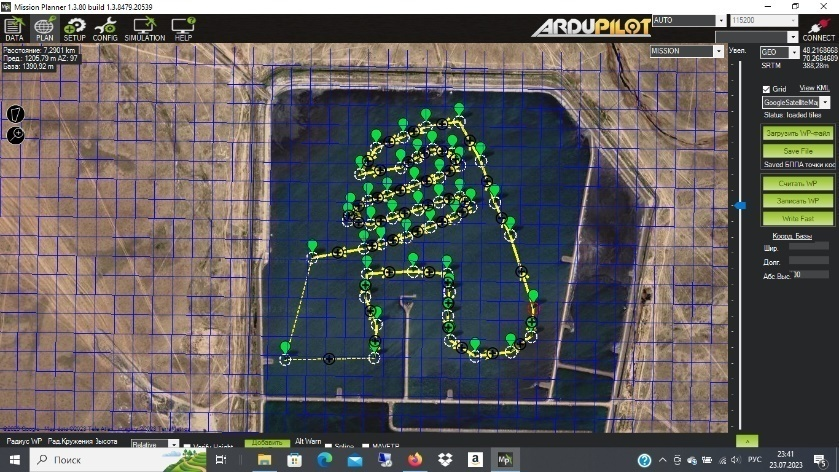
\includegraphics[width=0.8\textwidth]{assets/208}
	\caption*{}
\end{figure}

{\bfseries Рис. 1 -- Построение траектории в Mission Planner}

Важно отметить, что для успешного построения траектории и выполнения
автономного полета с помощью HEX Pixhawk 2.1 CUBE ORANGE+ также
необходимо обеспечить правильную калибровку и настройку всех датчиков и
устройств, используемых на БППА. Кроме того, при использовании
беспилотных плавательных аппаратов критически важно обеспечение
безопасности полетов и соблюдение всех нормативных норм и правил (Рис.
2).

\begin{figure}[H]
	\centering
	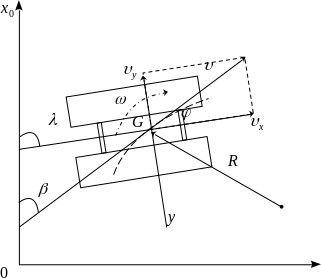
\includegraphics[width=0.8\textwidth]{assets/209}
	\caption*{}
\end{figure}

{\bfseries Рис. 2 -- Схема исследования траектории плавающего робота при
повороте}

Для анализа движения мобильного робота представляется необходимым ввести
системы координат, описывающее его движения. При этом используются две
системы координат: фиксированная \(X_{0}OY_{0}\). и подвижная XGY,
жестко связанная со станком. Оси стационарной системы координат
выбираются в качестве начальных так, чтобы в начальный момент времени
они совпадали с осями движущейся системы.

Угол \(\lambda\), образующийся между диаметральной плоскостью (ДП) и
осью \(X_{0}\), называется курсовым углом. Этот угол можно выразить
через другие углы, например:

Центральный угол сноса (\(\varphi\)), который измеряется между вектором
мгновенной скорости центра тяжести (ЦТ) робота и диаметральной
плоскостью.

Угол траектории (\(\beta\)) или угол скорости, который измеряется между
вектором скорости и \(X_{0}\) осью. Для оценки влияния течения на
управляемость плавающего робота анализируется их движение в двух
случаях: с течением и без течения. Это осуществляется путем построения
траекторий движения робота на основе исходных данных теста. Параметры
движения робота можно определить через проекцию скорости центра тяжести
на движущиеся оси и угловую скорость. Однако в некоторых ситуациях
удобнее использовать альтернативные кинематические параметры: модуль
скорости центра тяжести (│\(v\)│), угол сноса (\(\varphi\)) и угловую
скорость. Такая система параметров позволяет более удобно описывать
движение и анализировать его влияние на управляемость робота при
различных условиях течения {[}7{]}.

-- абсолютная скорость транспортного средства относительно системы
координат: угол траектории или угол скорости, измеренный между вектором
скорости и осью {[}8{]}.

v-- абсолютная скорость транспортного средства относительно системы
координат \(X_{0}OY_{0}\). : угол траектории или угол скорости,
измеренный между вектором скорости и осью \(X_{0}\) {[}7{]}.

\begin{longtable}[]{@{}
  >{\raggedright\arraybackslash}p{(\columnwidth - 2\tabcolsep) * \real{0.8955}}
  >{\raggedright\arraybackslash}p{(\columnwidth - 2\tabcolsep) * \real{0.1045}}@{}}
\toprule\noalign{}
\begin{minipage}[b]{\linewidth}\raggedright
\[X = \int_{0}^{t}v\cos(\beta)dt\]

\[Y = \int_{0}^{t}v\sin(\beta)dt\]
\end{minipage} & \begin{minipage}[b]{\linewidth}\raggedright
(1)
\end{minipage} \\
\midrule\noalign{}
\endhead
\bottomrule\noalign{}
\endlastfoot
\end{longtable}

В отсутствие потока (скорость потока равна нулю) траектория робота
подчиняется следующим принципам и уравнениям:

\begin{longtable}[]{@{}
  >{\raggedright\arraybackslash}p{(\columnwidth - 2\tabcolsep) * \real{0.8955}}
  >{\raggedright\arraybackslash}p{(\columnwidth - 2\tabcolsep) * \real{0.1045}}@{}}
\toprule\noalign{}
\begin{minipage}[b]{\linewidth}\raggedright
\[X = \int_{0}^{t}v\cos(\beta + \omega t)dt = \int_{}^{}\left( v_{x} - at \right)\cos(\varphi + \omega t)dt\]

\[Y = \int_{0}^{t}v\sin(\beta + \omega t)dt = \int_{}^{}\left( v_{y} - at \right)\sin(\varphi + \omega t)dt\]
\end{minipage} & \begin{minipage}[b]{\linewidth}\raggedright
(2)
\end{minipage} \\
\midrule\noalign{}
\endhead
\bottomrule\noalign{}
\endlastfoot
\end{longtable}

Эти уравнения описывают прямолинейное равномерное движение робота без
учета влияния потока. Таким образом, при отсутствии потока машина будет
двигаться прямолинейно со скоростью \(v\) под углом к положительному
направлению оси X.

Траектория катамарана под действием течения определяется следующим
образом:

\begin{longtable}[]{@{}
  >{\raggedright\arraybackslash}p{(\columnwidth - 2\tabcolsep) * \real{0.9063}}
  >{\raggedright\arraybackslash}p{(\columnwidth - 2\tabcolsep) * \real{0.0937}}@{}}
\toprule\noalign{}
\begin{minipage}[b]{\linewidth}\raggedright
\[X = \int_{}^{}v_{i}\cos(\beta + \omega t)dt = \int_{}^{}\left( \sqrt{v^{2} + v_{f}^{2} + v_{c}v_{t}\cos\left( \varphi_{f} \right)} \right)\cos(\beta + \omega t)dt\]

\[Y = \int_{}^{}v_{i}\sin(\beta + \omega t)dt = \int_{}^{}\left( \sqrt{v^{2} + v_{f}^{2} + v_{c}v_{t}\sin\left( \varphi_{f} \right)} \right)\sin(\beta + \omega t)dt\]
\end{minipage} & \begin{minipage}[b]{\linewidth}\raggedright
(3)
\end{minipage} \\
\midrule\noalign{}
\endhead
\bottomrule\noalign{}
\endlastfoot
\end{longtable}

При наличии течения абсолютная скорость \(v_{c}\) cотносительно системы
координат \(Х_{0}ОУ_{0}\) определяется, как показано на рисунке 3.

Результаты расчетной оценки влияния скорости течения на траекторию
движения катамарана с использованием программы Python.

\begin{figure}[H]
	\centering
	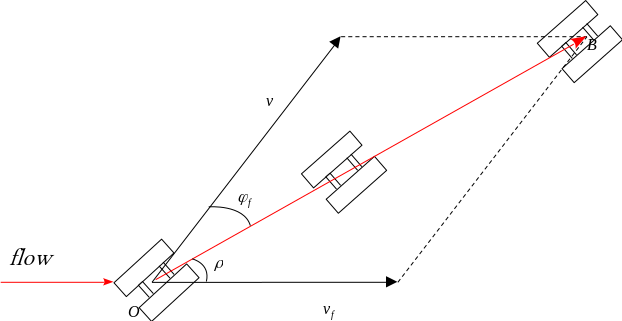
\includegraphics[width=0.8\textwidth]{assets/210}
	\caption*{}
\end{figure}

{\bfseries Рис. 3 -- С хема исследования траектории плавающего робота при
повороте под действием}

{\bfseries потока воды}

Для наглядности предположим, что мы хотим рассчитать траекторию
катамарана в течение первых 10 секунд (без учета и без учета течения)
(Рис. 4).

\begin{figure}[H]
	\centering
	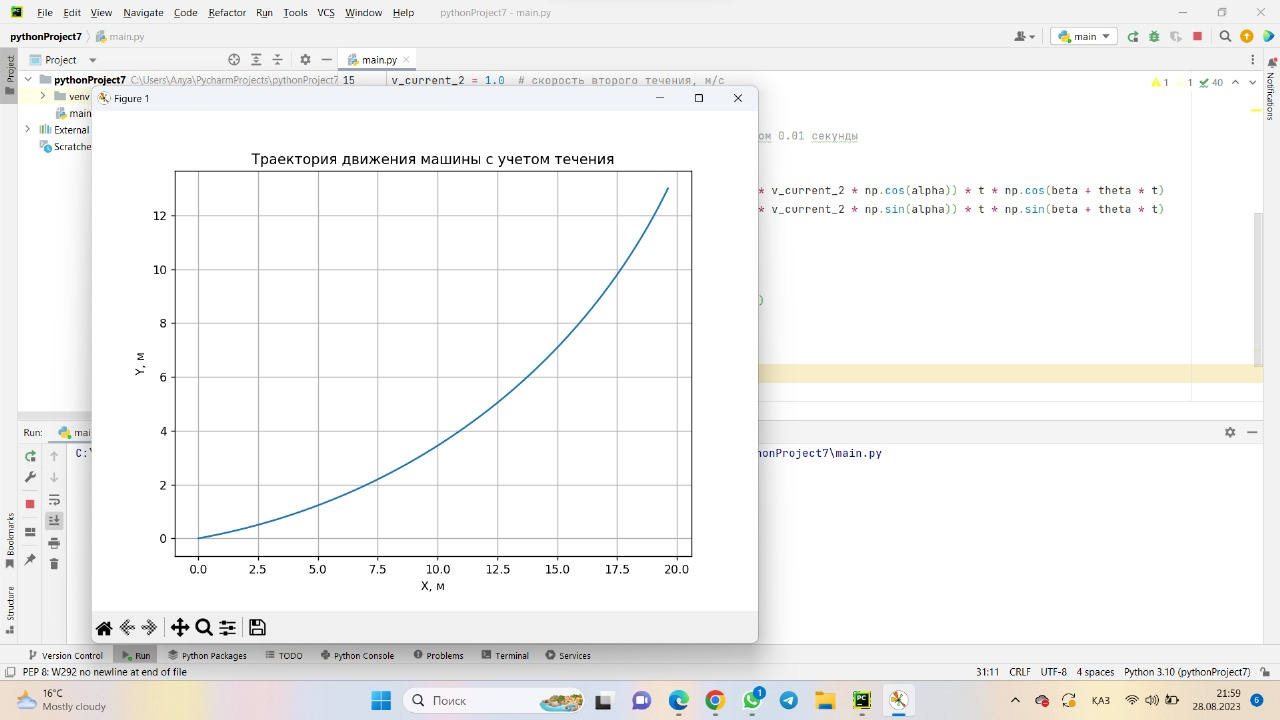
\includegraphics[width=0.8\textwidth]{assets/211}
	\caption*{}
\end{figure}

{\bfseries Рис. 4 -- Траектория катамарана в течение первых 10 секунд (без
учета и без учета течения)}

Для расчета траектории катамарана с учетом скорости потока воды можно
модифицировать уравнения движения с учетом дополнительной скорости,
вызванной течением. Вам нужно будет сложить векторы скорости плавания и
вектор скорости потока, чтобы определить конечную скорость автомобиля:
По оси OX и OY. если масса машины 75 кг, длина 1,57 м, ширина 0,515 м,
высота 0,3, скорость плавания 0,5 м/с, угол сноса 0,1 рад., угол
скорости 0,2 рад., относительный радиус поворота 0,75 м., угол скорости
0,05 рад/с., скорость первого потока 1,4 м/с, скорость второго потока 1
м/с. Начальная координата 0,0.

\emph{Разработка программного обеспечения для получения 2D, 3D карт
дна.} Полученные данные с борта, в частности от эхолокационного
устройства (данные о глубине) и HEX Pixhawk 2.1 CUBE ORANGE+ (данные
GPS, данные о состоянии, данные о траектории), передаются в удаленный
командный центр (компьютер). Данные, полученные от HEX Pixhawk 2.1 CUBE
ORANGE+, отправляются в Mission Planner для мониторинга данных в
реальном времени, таких как координаты GPS, высота, скорость, состояние
батареи и другие параметры {[}9-10{]}. Эти данные можно сохранить в
текстовый файл и отправить на веб-сервер для последующего сохранения в
базе данных MySQL. Далее с помощью разработанного программного кода на
Python и его библиотек данные обрабатываются и визуализируются в 2D и 3D
графике. Для быстрой обработки используется библиотека Numpy,
позволяющая конвертировать данные в удобный для анализа массив.
Созданный таким образом массив визуализируется с помощью библиотеки
plotly. Для создания 2D и 3D графики используется экспресс-инструмент,
который, получая ранее созданный массив данных, создает динамическое
окно с графиками (Рис. 5). Затем Python создает html-файл с готовыми
графиками. В это окно добавлены CSS-классы для более удобного
интерфейса, с которым будет взаимодействовать пользователь (Рис. 6).
Готовый html-файл отправляется клиенту приложения, где пользователь
может его видеть и взаимодействовать с ним. На рисунке 5 3D карта дна
хвостохранилища Жайремского горно-обогатительного комбината. Объект был
исследован несколько раз для большей точности данных.

\begin{figure}[H]
	\centering
	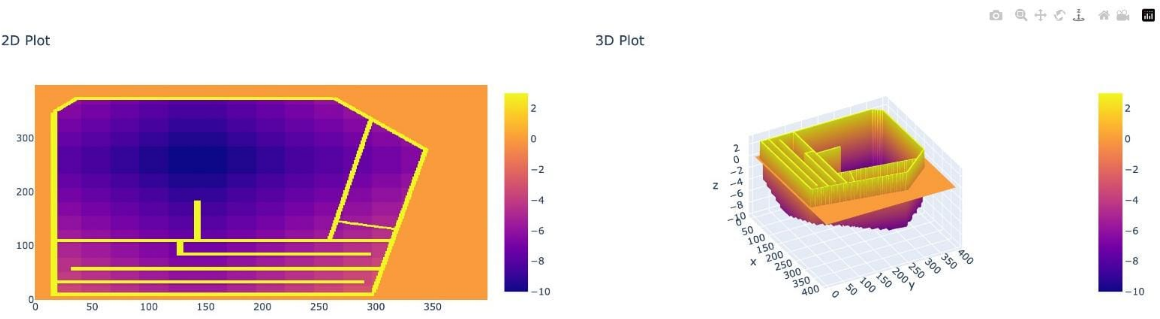
\includegraphics[width=0.8\textwidth]{assets/212}
	\caption*{}
\end{figure}

{\bfseries Рис. 5 -- 2D, 3D карта дна хвостохранилища Жайремского
горно-обогатительного комбината}

\begin{figure}[H]
	\centering
	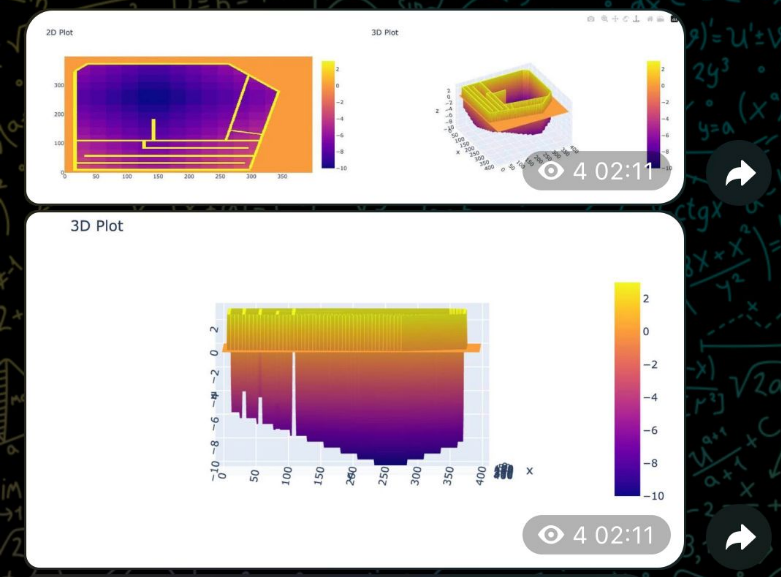
\includegraphics[width=0.8\textwidth]{assets/213}
	\caption*{}
\end{figure}

{\bfseries Рис. 6 -- Телеграм бот}

По результатам испытаний робототехнического комплекса получены данные об
ошибке движения робота в системе координат, которая составляет примерно
0,2 метра по оси x и 0,1 метра по оси y. Во время испытаний температура,
влажность, уровень кислорода (O2) и концентрация частиц были практически
постоянными. Также известно, что средняя глубина хвостохранилища
составляет 4,56 метра.

На основании этих данных были произведены расчеты объема воды. Для этого
были замерены площади водосборов различных участков: площадь водосбора
участка баритового хвостохранилища - 2,5 км2, площадь водосбора участка
баритового хвостохранилища вместе с участком фильтрации - 0,38 км2.
Также установлено, что в пруду-окислителе скопилось 1,85 млн м3 воды,
что соответствует уровню воды на отметке 392,55 метра.

Результаты расчетов позволили установить следующие факты:

В первом полугодии 2021 года был «нулевой» баланс без сброса излишков в
пруд-испаритель. Этого удалось добиться за счет замачивания основания и
заполнения участков хвостохранилища, что предотвратило сброс воды.

За последующий период до конца 2023 года зафиксировано превышение
оборотной воды в пределах от 6704,443 до 24593,282 млн м3, которая
сбрасывалась в пруд-испаритель. Это позволило контролировать уровень
воды в системе и избежать перелива.

Также установлено, что площадь и объем прудов-отстойников участков
хвостохранилища и пруда-окислителя обеспечивают:

Достаточное освещение оборотной воды, возвращаемой на завод в
технологическом процессе, позволяет повторно использовать эту воду.

Возможность складирования объема хвостов, поступающих в пруды-отстойники
в течение года, что способствует эффективному обращению с отходами.

Натурные эксперименты, проведенные с использованием мобильного
роботизированного комплекса, позволили сделать вывод, что МРК
обеспечивает стабильную и надежную передачу данных. Преодоление помех,
возникающих на выходах датчиков, было достигнуто за счет внедрения схем
развязки, что значительно улучшило качество сигнала и обеспечило более
точные измерения. Программное обеспечение, предназначенное для
эффективного контроля и мониторинга функций работы системы при
использовании на персональном ноутбуке. Это обеспечивает полный спектр
функциональных возможностей предлагаемой системы и обеспечивает ее
высокую практичность в реальных условиях эксплуатации. Следует отметить,
что внедрение датчика воды в БППА дает водникам уникальную возможность
осуществлять непрерывный мониторинг и контроль параметров качества воды
на уязвимых и стратегически важных участках хвостохранилищ и водоемов.
Такой подход значительно повышает эффективность и результативность
управления водными ресурсами, способствуя более рациональному и
обоснованному принятию решений в этой области.

{\bfseries Результаты и обсуждение.} Рисунок 1 демонстрирует графическое
представление траекторий полета БППА для разных сценариев. На рисунке 5
представлена 3D карта дна хвостохранилища Жайремского
горно-обогатительного комбината, которая была визуализирована в
результате ряда экспериментов с применением разработанного
исследовательской группой проекта AP09058557 и авторами статьи МРК, над
хвостохранилищем. Объект был исследован несколько раз для большей
точности данных.

Исследование направлено на разработку и апробацию методов планирования
траекторий для БППА с использованием программного пакета Mission
Planner. Основной целью было улучшение точности и эффективности
управления беспилотными аппаратами.

Наиболее значимые результаты включают улучшение времени полета и
точности навигации при использовании новых алгоритмов планирования
траекторий. Сравнение с другими исследованиями показывает сопоставимые
или более высокие показатели эффективности разработанных методов. Однако
проблемные зоны включают необходимость дальнейшей оптимизации алгоритмов
для учета разнообразных условий полета.

В данной работе был представлен процесс построения траектории полета для
беспилотных аппаратов с использованием HEX Pixhawk 2.1 CUBE ORANGE+ и
программного пакета Mission Planner. Этот процесс включает в себя учет
различных параметров полета, таких как высота, скорость и курс, и
позволяет эффективно управлять беспилотными аппаратами в соответствии с
заданными целями. Основное внимание уделено безопасности и настройке
датчиков и устройств, необходимых для автономного полета. Проведенный
анализ движения мобильного робота, включая оценку углового ускорения и
скорости с учетом воздействия течения, позволяет более точно планировать
маршруты и управлять беспилотными аппаратами в различных условиях.
Дополнительно, рассмотрены методы разработки программного обеспечения
для получения и обработки данных о глубине морского дна с использованием
HEX Pixhawk 2.1 CUBE ORANGE+ и эхолокационного устройства. Этот подход
открывает новые перспективы для исследования морских ресурсов с высокой
точностью и безопасностью. Таким образом, представленная методика и
результаты работы имеют важное значение для разработки и управления
беспилотными аппаратами, а также для проведения исследований морского
дна и его ресурсов. Дальнейшие исследования в этой области могут
включать расширение функциональности программного обеспечения, а также
углубленный анализ влияния различных параметров на эффективность
управления беспилотными аппаратами.

{\bfseries Выводы\emph{.}} В ходе исследования были рассмотрены методы
планирования траекторий для беспилотных аппаратов с использованием
программного пакета Mission Planner. Полученные результаты позволяют
сделать вывод о повышении точности и эффективности управления БППА в
различных сценариях полета. Были изучены специализированные программные
пакеты и алгоритмы для планирования траекторий полета беспилотных
аппаратов. Разработаны и апробированы методы построения траекторий с
использованием оборудования HEX Pixhawk 2.1 CUBE ORANGE+ и программного
пакета Mission Planner. Проведен анализ движения мобильных роботов с
учетом воздействия течения, что позволило определить оптимальные
стратегии управления в различных условиях. Полученные результаты
подтверждают гипотезу о том, что применение специализированных методов
планирования траекторий повышает эффективность управления беспилотными
аппаратами. Таким образом, разработанные методы и алгоритмы имеют
потенциал для широкого применения в области автономных систем и могут
быть использованы для улучшения точности и эффективности управления
беспилотными аппаратами.

\emph{{\bfseries Финансирование.} Работа выполнена при поддержке гранта МОН
РК в рамках проекта AP09058557 по договору No63-КМУ2 от 24 февраля 2021
года.}

{\bfseries Литература}

\begin{enumerate}
\def\labelenumi{\arabic{enumi}.}
\item
  Shubhani Aggarwal, Neeraj~Kumar. Path planning techniques for unmanned
  aerial vehicles: A review, solutions, and challenges // Computer
  Communications. - 2020. -- Vol. 149. - P. 270-299. DOI:
  10.1016/j.comcom.2019.10.014.
\item
  Faiyaz Ahmed, J.C. Mohanta, Mohd. Nayab Zafar. Development of smart
  quadcopter for autonomous overhead power transmission line inspections
  // -- 2022. -- Vol. 51(1). -P. 261-268. DOI:
  10.1016/j.matpr.2021.05.271
\item
  How to connect a PixHawk Cube or similar system - a simple overview.
  --URL: https://www.youtube.com/watch?v=tIE8IN71UFI. (date of
  application15.06.2024)
\item
  All the confusing names in \textquotesingle Pixhawk\textquotesingle{}
  explained (Mission Planner, PX4, Ardupilot Pixhawk etc.) --URL:
  https://www.youtube.com/watch?v=0vBXFjhw-5M. (date of
  application15.06.2024)
\item
  Khosyi\textquotesingle In, M., Budisusila, E.N., Dwi Prasetyowati
  S.A., Suprapto B.Y.; Nawawi Z. Design of Autonomous Vehicle Navigation
  Using GNSS Based on Pixhawk 2.1 // International Conference on
  Electrical Engineering, Computer Science and Informatics
  (EECSI)\emph{.} -- 2021. -P. 175 -- 180. DOI:
  10.23919/EECSI53397.2021.9624244.
\item
  Mission Planner Overview, 2021, {[}online{]} Available. --URL:
  htt://ardupilot.org/planner/docs/mission-planner-overview.html. (date
  of application15.06.2024)
\item
  Myasischev, O. O., Lienkov, S. V., Ovcharuk, V. V., Tolok, I.,
  Lytvynenko, N., Zinchyk, A. G., \& Lytvynenko, O. I. Large-capacity
  quadcopter's designing on the controllers of the pixhawk cube family.
  75. -2022. --P. 108-118. DOI: 10.17721/2519-481x/2022/75-11
\item
  S. Fujita and S. Mae Causes and Nature of ice-sheet radio-echo
  internal reflection estimated from the dielectric properties of ice //
  Annals of glaciology. -1994. -Vol. 20. -P. 80-86.
\item
  Nicolas A.; Olmedo and Michael G. Lipsett. 2016. Design and field
  experimentation of a robotic system for tailings characterization //
  Journal of Unmanned Vehicle Systems. --Vol. 4(3). --P. 169-192. DOI
  10.1139/juvs-2015-0034.
\item
  Lienkov, S., Myasischev, A. A., Ovcharuk, V., Lenkov, E., \&
  Lytvynenko, N.. Development of Multifunctional Rotary UAV Based on
  Pixhawk Family Flight Controllers. -2023. --Vol. 18(1). DOI:
  10.3849/aimt.01752
\end{enumerate}

\emph{{\bfseries Сведения об авторах}}

Жартыбаева М.Г.-PhD., Евразийский национальный университет им. Л. Н.
Гумилева, Астана, Казахстан, e-mail: makkenskii@mail.ru;

Алинова А.Д.-Евразийский национальный университет им. Л. Н. Гумилева,
Астана, Казахстан, e-mail: alinova-aida@mail.ru;

Оралбекова Ж.О. -PhD, Евразийский национальный университет имени Л.Н.
Гумилева, Астана, Казахстан, e-mail: oralbekova@bk.ru;

Тюлепбердинова Г.А.-к.ф.-м.н., доцент, Казахский национальный
университет им. Аль-Фараби, Алматы, Казахстан, e-mail:
tyulepberdinova@gmail.com;

Жамишева Н.М.-\/-«Институт законодательства и правовой информации
Республики Казахстан» Министерства юстиции Республики Казахстан, главный
специалист отдела поддержки информационных систем, Астана, Казахстан,
e-mail: nuray\_zhamisheva33@gmail.com.

\emph{{\bfseries Information about the authors}}

Zhartybayeva M.G. -PhD., L. N. Gumilyov Eurasian National University,
Astana, Kazakhstan, e-mail: makkenskii@mail.ru;

Alinova A/D.- L. N. Gumilyov Eurasian National University, Astana,
Kazakhstan, e-mail: alinova-aida@mail.ru;

Oralbekova Zh. O. -Ph.D., L.N. Gumilyov Eurasian national university,
Astana, Kazakhstan, e-mail: oralbekova@bk.ru;

Tyulepberdinova G.A.- PhD, associate professor, Al-Farabi Kazakh
National University, Almaty, Kazakhstan, e-mail:
tyulepberdinova@gmail.com;

Zhamisheva N.M. - Institute of Legislation and Legal information of the
Republic of Kazakhstan" Ministry of Justice of the Republic of
Kazakhstan, Chief specialist of the information systems support
department, Astana, Kazakhstan, e-mail: nuray\_zhamisheva33@gmail.com.




